\chapter{Methylamine survey in low mass star-forming regions
  \label{chap:LMSFRs}}

\section{Review of low mass star-forming region}
\section{Analysis}

\section{IRAS 16293}
\subsection{Observation data}
\subsection{Results}

\begin{figure}[H]
  \centering
  \includegraphics[width=0.7\textwidth]{LMSFR/IRAS16293_mom0.eps}
  \caption{Integrated intensity map around 247.362 GHz. The white contours represent the 1.3 mm continuum map, where the contour levels are 10 \%, 30 \%, 50 \%, 70 \%, 90 \% of the peak intensity.}
  \label{IRAS16293_mom0}
\end{figure}

\begin{figure}[H]
  \centering
  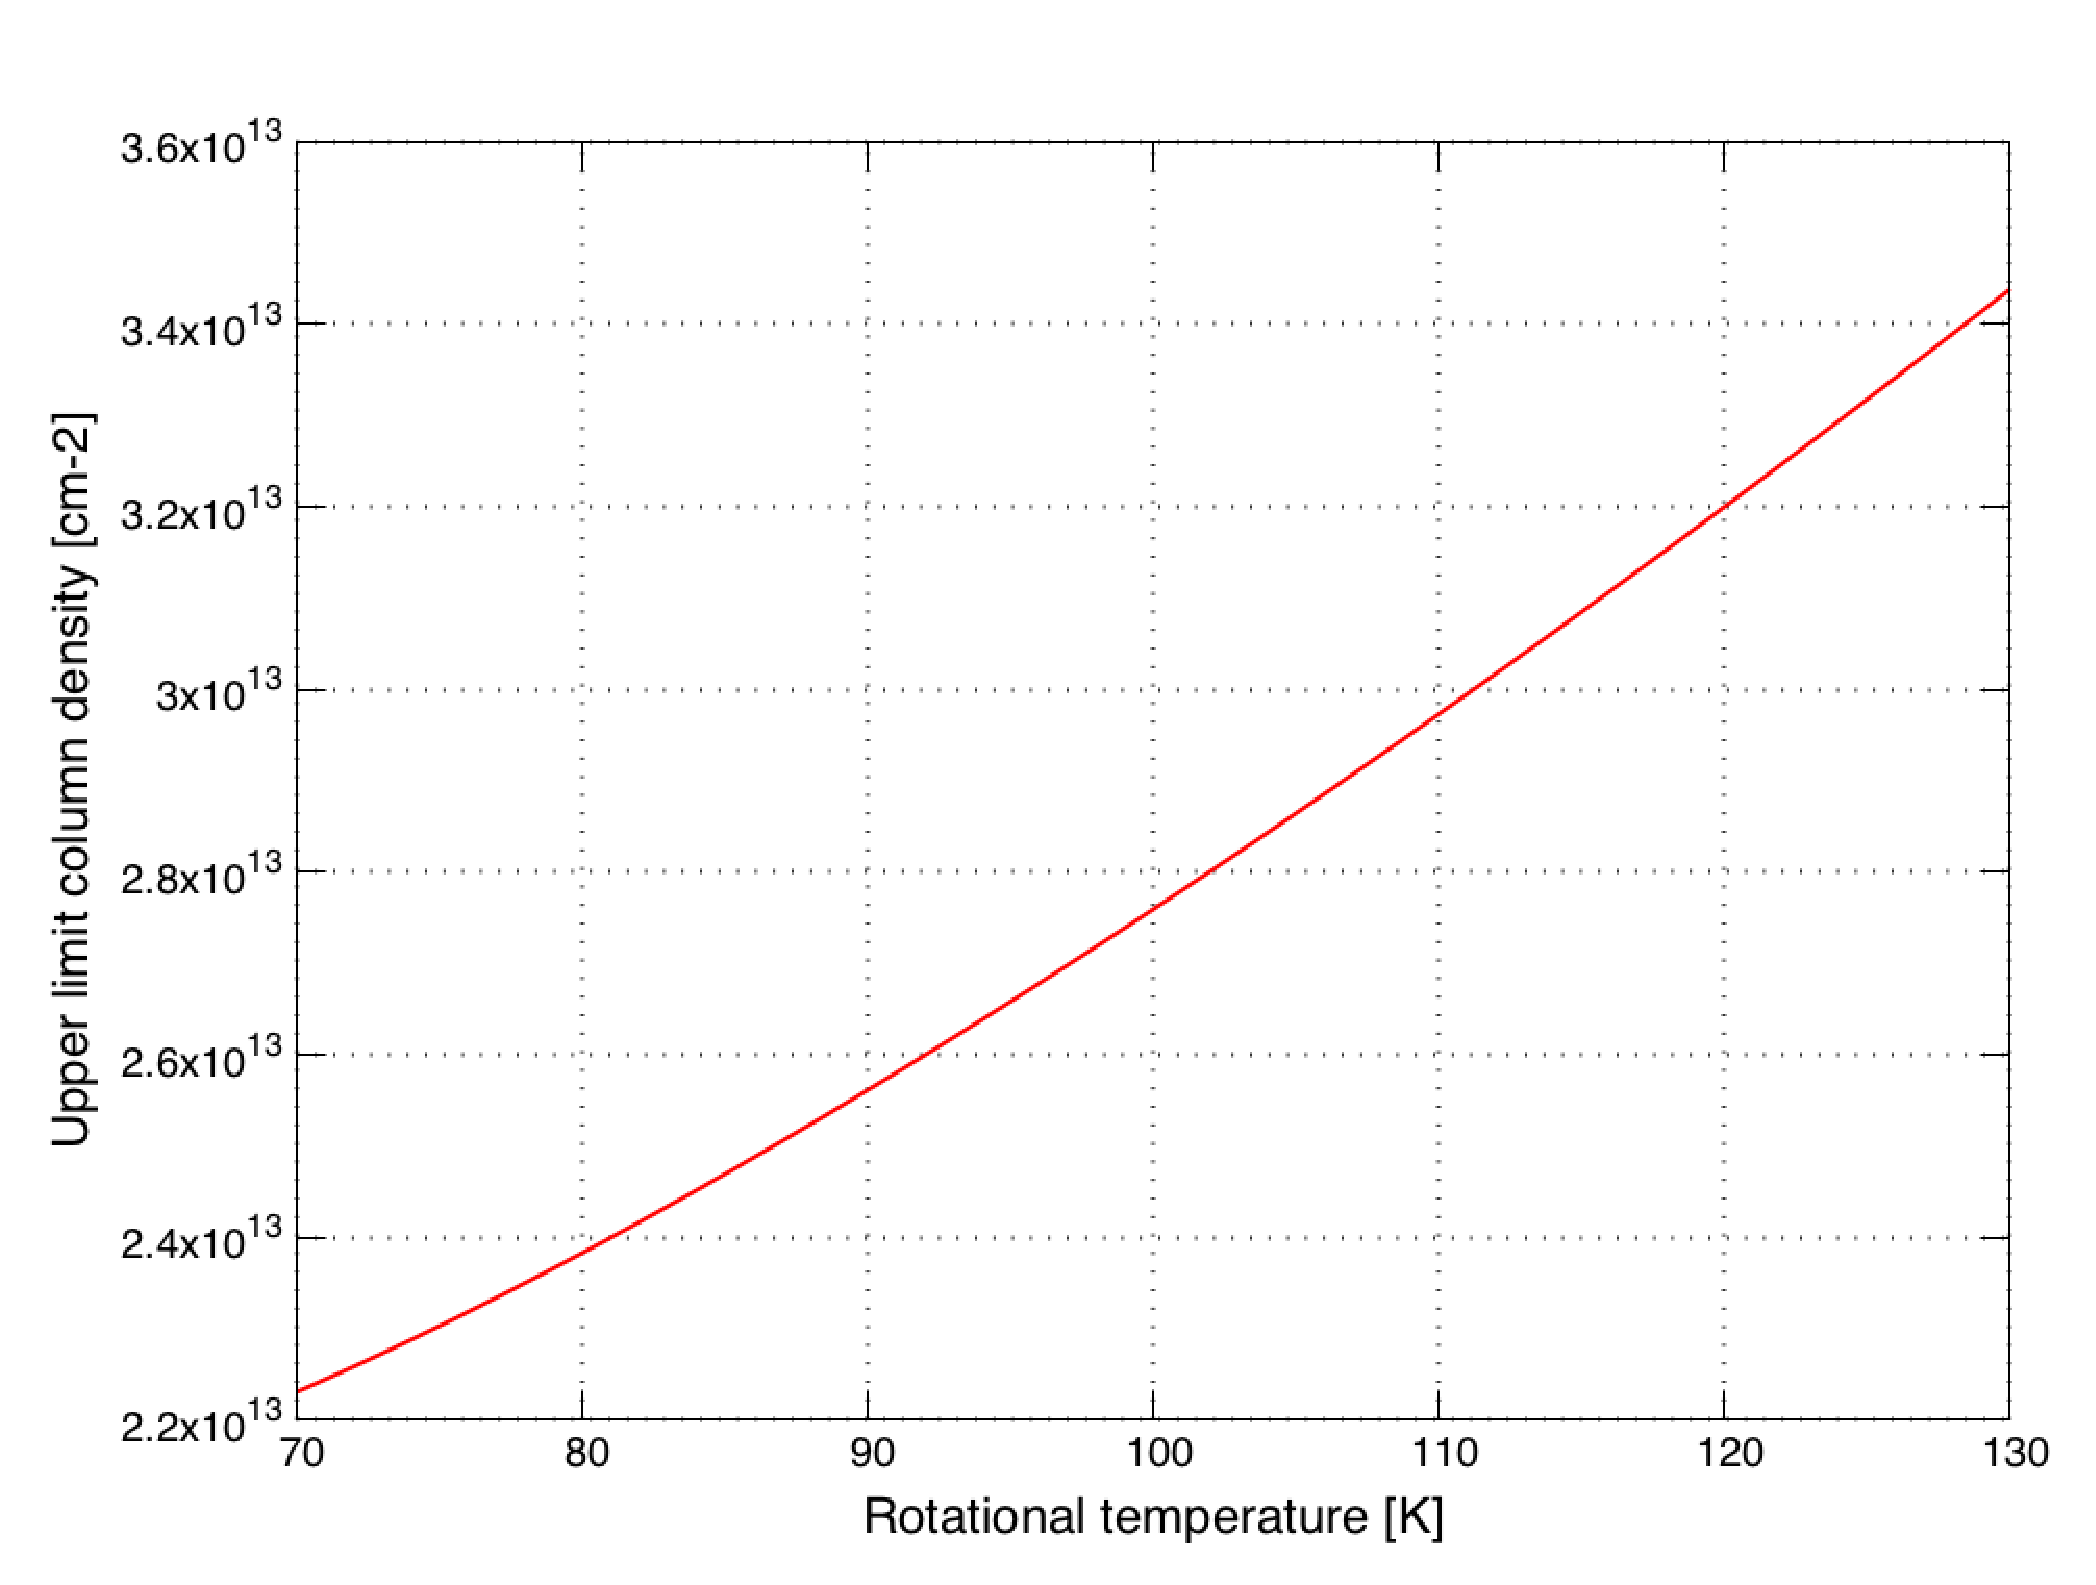
\includegraphics[width=0.7\textwidth]{LMSFR/IRAS16293.eps}
  \caption{Upper limit column density for the strongest CH$_{3}$NH$_{2}$ transition
  ($7_{2}E_{1-1} \rightarrow 7_{1}E_{1-1}$) as function of T$_{\textrm{rot}}$. A 3$\sigma$ value of 
  11.4 mJy beam$^{-1}$ is used.}
  \label{IRAS16293_MA}
\end{figure}


%\subsubsection{Transitions}
%\subsubsection{Integrated intensity map}
%\subsubsection{Upper limit column density}

\section{L483}
\subsection{Observation data}
\subsection{Results}

\begin{figure}[H]
  \centering
  \includegraphics[width=0.7\textwidth]{LMSFR/L483_mom0.eps}
  \caption{Integrated intensity map around 217.079 GHz. The white contours represent the 1.3 mm continuum map, where the contour levels are 10 \%, 30 \%, 50 \%, 70 \%, 90 \% of the peak intensity.}
  \label{L483_mom0}
\end{figure}

\begin{figure}[H]
  \centering
  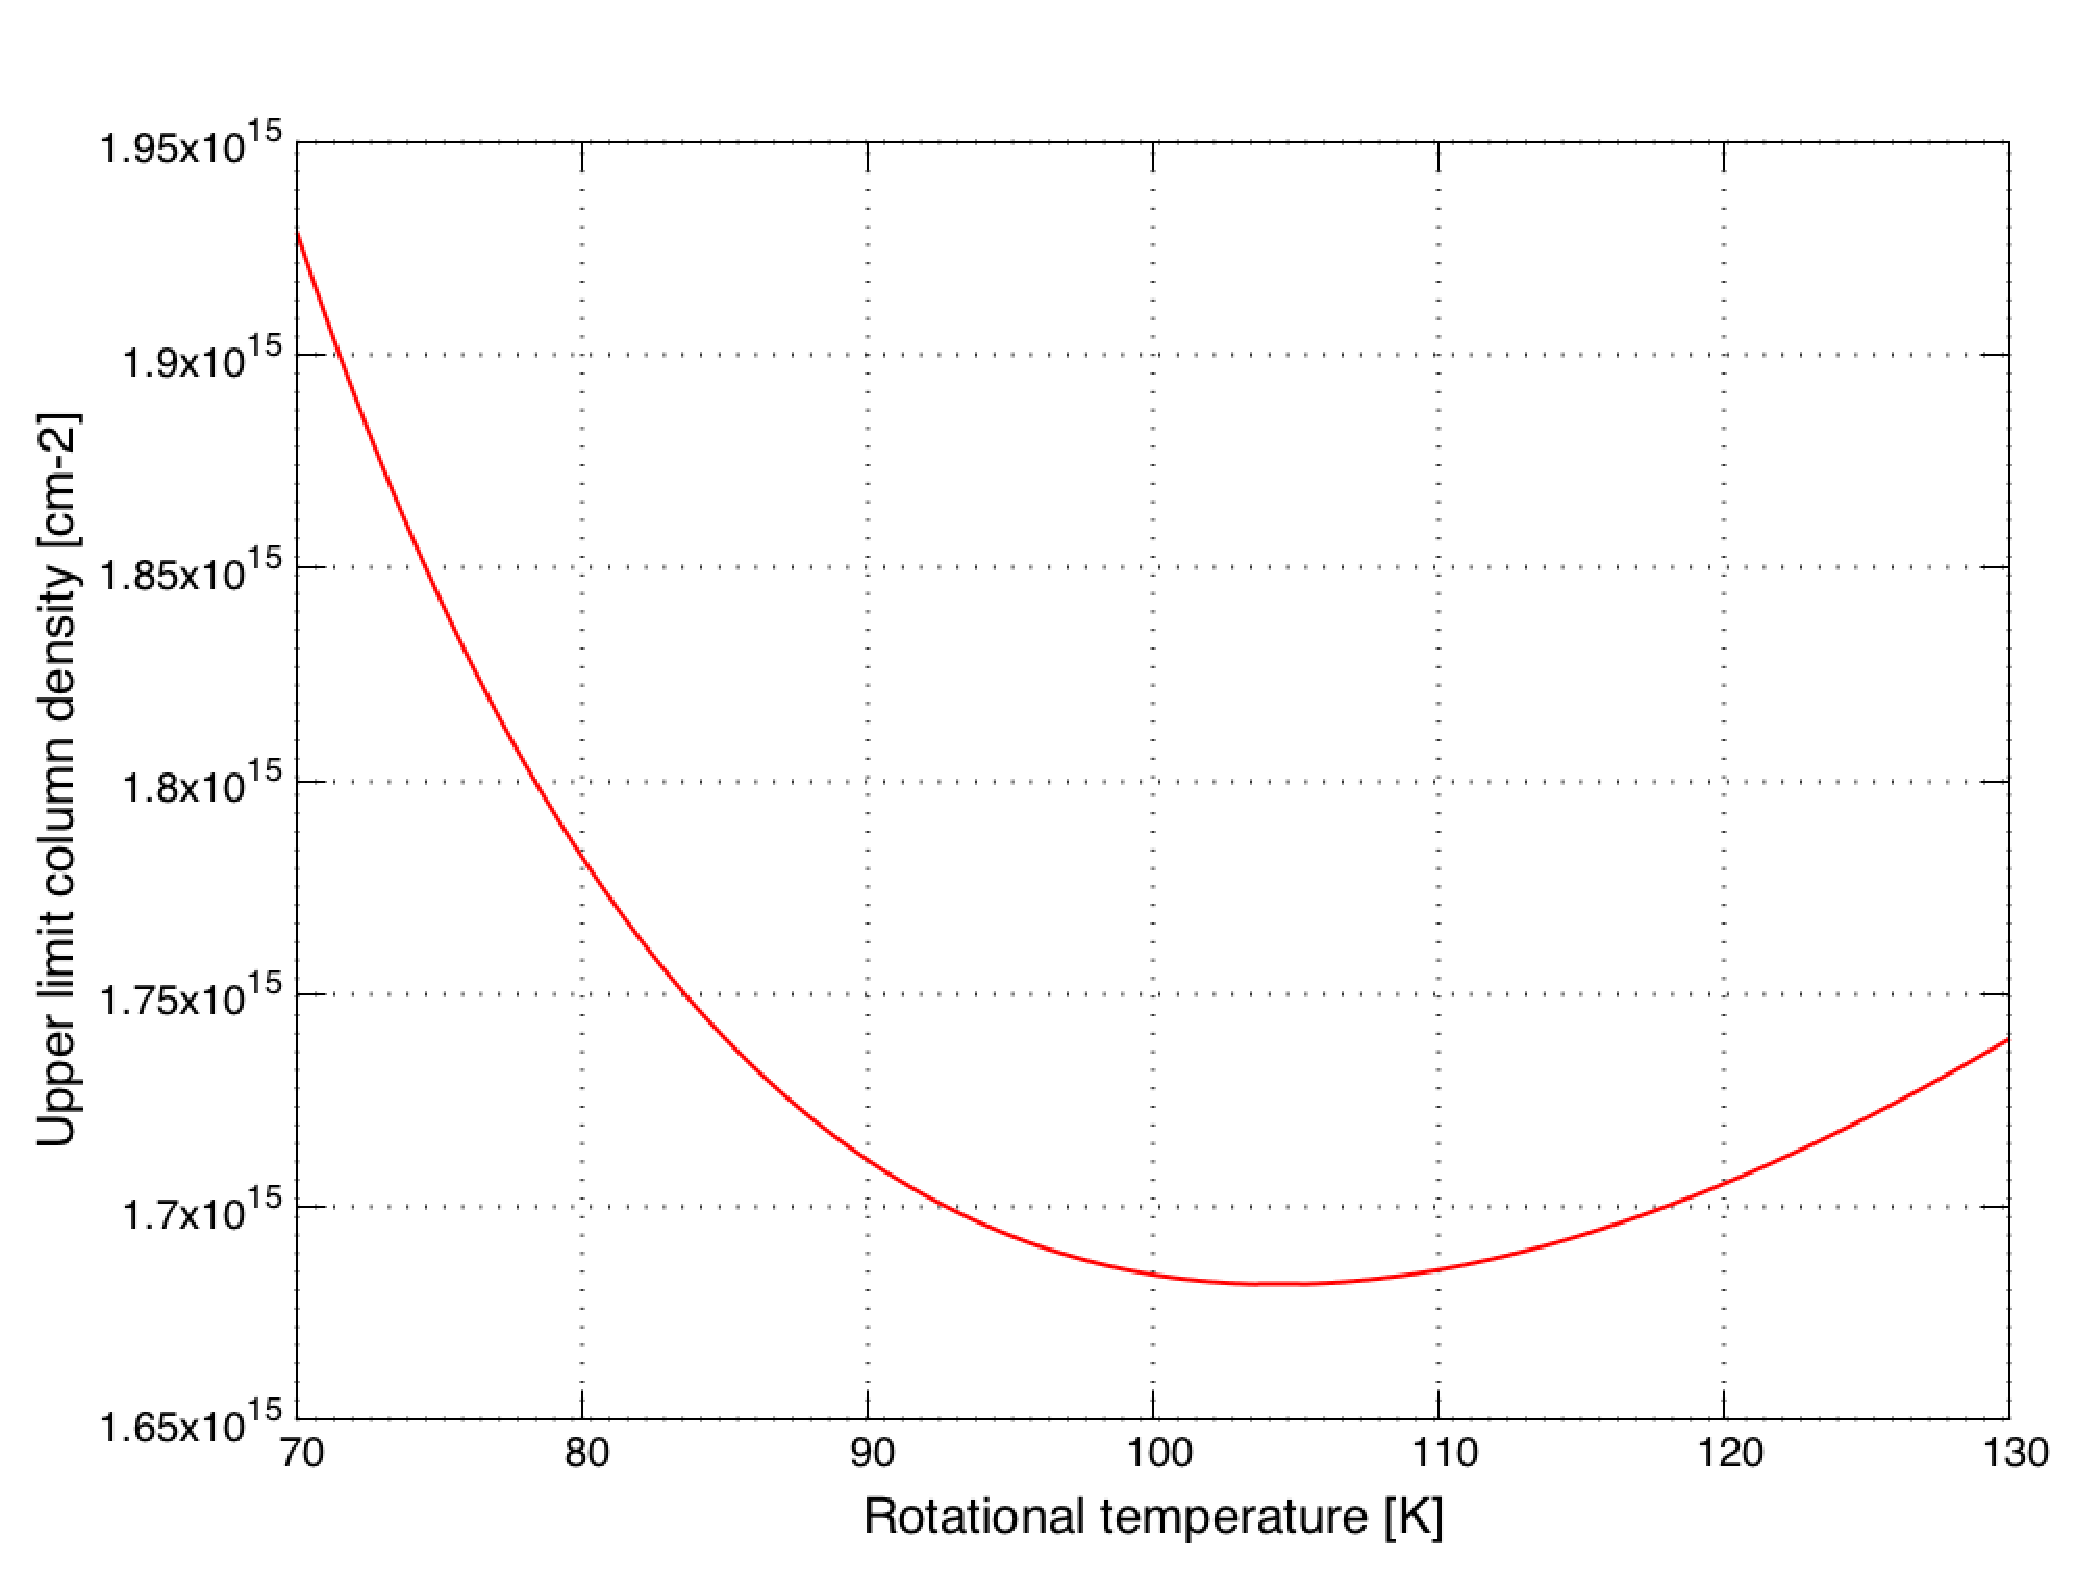
\includegraphics[width=0.7\textwidth]{LMSFR/L483.eps}
  \caption{Upper limit column density for the strongest CH$_{3}$NH$_{2}$ transition
  ($11_{2}A_{1} \rightarrow 11_{2}A_{2}$) as function of T$_{\textrm{rot}}$. A 3$\sigma$ value of 
  22.5 mJy beam$^{-1}$ is used.}
  \label{L483_MA}
\end{figure}


%\subsubsection{Transitions}
%\subsubsection{Integrated intensity map}
%\subsubsection{Upper limit column density}